\documentclass[11pt]{article}
\usepackage[utf8]{inputenc}
\usepackage{amsmath}
\usepackage{graphicx}
\usepackage{blindtext}
\usepackage{listings}
\usepackage{hyperref}
\usepackage{longtable}
%Gummi|065|=)
\title{\textbf{Proyecto Parcial 2 - biseccion}}
\author{Brian de Jesús Herberth Guerrero\\
		A00398663}
\date{11 Abril 2016}
\begin{document}

\maketitle
\tableofcontents
\clearpage

\section{Introduccion}
El metodo de biseccion es un algoritmo de busqueda de raices que se  se basa en el teorema del valor intermedio el cual trabaja dividiendo el intervalo a la mitad y seleccionando el subintervalo que tiene la raíz. En otras palabras el metodo dividira a la mitad un intervalo \emph{[a,b]} en repetidas ocasiones hasta encontrar la mitad de la solucion, \emph{m}.Resolucion del algoritmo:\\

\begin{flushleft}
\textbf{Paso 1:}
Elegir los valores iniciales Xa y Xb, de tal forma de que la función cambie de signo:

\begin{equation*}
  f(Xa)f(Xb) < 0
\end{equation*}

\textbf{Paso 2:}
La primera aproximación a la raíz se determina con la fórmula del punto medio de esta forma:
\begin{equation*}
  Xpm=\frac{Xa+Xb}{2}
\end{equation*}

\textbf{Paso 3:}
Realizar las siguientes evaluaciones para determinar el intervalo de la raíz:
\begin{itemize}
  \item Si f(Xa)f(Xb) menor que 0, entonces la solución o raíz está entre Xa y Xpm, y Xb pasa a ser el punto medio (Xpm).
  \item Si f(Xa)f(Xb) > 0, entonces la solución o raíz está fuera del intervalo entre Xa y el punto medio, y Xa pasa a ser el punto medio (Xpm).
\end{itemize}

\end{flushleft}
\clearpage

\subsection{Aplicaciones}
Algunas aplicaciones en la ingenieria y ciencias son:
\begin{itemize}
\item Ingenieria Electrica en la creacion de un circuito electrico.
\item Ingenieria industrial en el calculo de error en una produccion.
\item Disenio asistido por copuntadora para la renderizacion.
\item Ingenieria Civil para la mecanica de solidos.
\item Ganaderia en el calculo de produccion de leche en una granja.
\item Ingenieria Petrolera en la optimisacion de procesos del crudo(petroleo).
\end{itemize}

\subsection{Videos}

En las siguientes ligas se pueden encontrar videos acerca de biseccion:
\begin{itemize}
\item \url{https://www.youtube.com/watch?v=z_GUatdKXzo}
\item \url{https://www.youtube.com/watch?v=0WPixuL6AZU}
\item \url{https://www.youtube.com/watch?v=MUCwZKPntXg}
\end{itemize}

\clearpage
\section{Caso de estudio}
Para esta caso de estudio se aplicara la siguiente ecuacion:

\begin{equation*}
  x^4+3x^3-2
\end{equation*}

\subsection{Dataset}

Se utilizara la siguiente tabla:

\begin{center}
\begin{tabular}{ |c|c| } 
\hline
X & Y \\
\hline
-2 & 10  \\ 
-1 & -4  \\ 
0 & -2  \\ 
1 & 2 \\ 
2 & 38  \\ 
\hline
\end{tabular}
\end{center}

\subsection{Graficos}

Utilizando la herramienta gnuplot se utlizaron las siguiente lineas de codigo como resultado la siguiente imagen:

\begin{itemize}
  \item set terminal png transparent nocrop enhanced size 450,320 font "arial,8" 
  \item set output 'caso.png'
  \item set key bmargin center horizontal Right noreverse enhanced autotitle box lt black linewidth 1.000 dashtype solid
  \item set samples 400, 400
  \item set title "Simple Plots"
  \item set title  font ",20" norotate
  \item plot [-2:2] (x**4)+(3*(x**3))-2
\end{itemize}

\clearpage

\begin{figure}[htp]
\centering
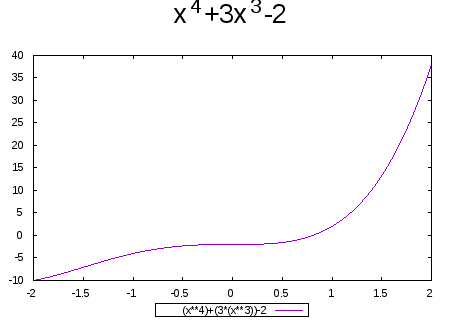
\includegraphics[width=10cm]{caso.png}
\label{fig:lion}
\end{figure}


\section{Experimento}

Se creo en c++ un programa en el cual se comprobo la funcion y  el metodo de biseccion:

\lstinputlisting{proyecto.cpp}
\clearpage
\subsection{Pruebas}
Se ejecuto con los siguientes comandos:
\begin{itemize}
\item g++ -o proyecto proyecto.cpp
\item ./protecto
\end{itemize}

\subsection{Graficacion con gnuplot}

\begin{figure}[htp]
\centering
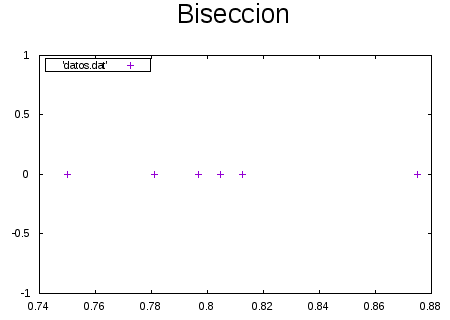
\includegraphics[width=10cm]{comparacion.png}
\label{fig:lion}
\end{figure}

\subsection{Validacion}

Se encontro en datos.dat la ubicacion exact de su interseccion con x en la ecuacion: 

\begin{equation*}
  x^4+3x^3-2
\end{equation*}
\clearpage
\section{Repositorio}

Se creo un repositorio en Github en las cuales contienen los siguientes archivos:


\begin{enumerate}
  \item proyecto.tex - archivo en latex del proyecto
  \item proyecto.pdf - pdf generado con pdflatex
  \item proyecto.cpp - codigo fuente del programa en C++
  \item datos.dat - archivo de datos generado por el programa
  \item caso.png y grafica.png -graficas generados con gnu-plot
\end{enumerate}

\section{Conclusiones}
El método de bisección es un algoritmo de búsqueda de raíces que trabaja dividiendo el intervalo a la mitad y seleccionando el subintervalo que tiene la raíz. Con este metodo tambien podremos encontar el punto en x por donde pasa la funcion al graficar si es que existe.

\end{document}
